%% annotation_pipelines.tex
%% Author: Leighton Pritchard
%% Copyright: James Hutton Institute
%% A brief description of gene prediction, as an illustrative example

% SUBSECTION: Annotation Pipelines
\subsection{Prokaryotic Annotation Pipelines}

% Prokaryotic annotation pipelines
\begin{frame}
  \frametitle{Prokaryotic Annotation Pipelines\footnote{\tiny{\href{http://dx.doi.org/10.1093/bib/bbs007}{Richardson and Watson (2012) \textit{Brief. Bioinf.} \textbf{14}:1-12 doi:10.1093/bib/bbs007}}}}
  Many choices, including \texttt{RAST}\footnote{\tiny{\href{http://dx.doi.org/10.1186/1471-2164-9-75}{Aziz \textit{et al}. (2008) \textit{BMC Genomics} \textbf{9}:75 doi:10.1186/1471-2164-9-75}}}, \texttt{PROKKA}\footnote{\tiny{\href{http://dx.doi.org/10.1093/bioinformatics/btu153}{Seemann (2014) \textit{Bioinformatics} \textbf{30}:2068-2069 doi:10.1093/bioinformatics/btu153}}}, \texttt{BaSYS}\footnote{\tiny{\href{http://dx.doi.org/10.1093/nar/gki593}{Van Domselaar \textit{et al}. (2005) \textit{Nuc. Acids Res.} \textbf{33}:W455-W459 doi:10.1093/nar/gki593}}}, etc.\\
  Often perform both CDS/feature calling and functional prediction.\\
  Two broad approaches:
  \begin{enumerate}
    \item Heavyweight: maintain database and resource, often annotating by homology, e.g. \texttt{RAST}
    \item Lightweight: chain together multiple third-party packages, e.g. \texttt{PROKKA}
  \end{enumerate}
  Pipelines take a lot of tedium (and control) out of annotating bacterial genomes, but have the same issues as every other prediction tool.
\end{frame}

% PROKKA
\begin{frame}
  \frametitle{PROKKA\footnote{\tiny{\href{http://dx.doi.org/10.1093/bioinformatics/btu153}{Seemann (2014) \textit{Bioinformatics} \textbf{30}:2068-2069 doi:10.1093/bioinformatics/btu153}}}}
  \begin{columns}
    \begin{column}{5cm}
      \begin{itemize}
        \item Lightweight, and fast. 
        \item Runs locally. (5Mbp genome takes $\approx$10min on my desktop; more detailed ncRNA prediction takes $\approx$20min)
        \item Flexible: built-in databases can be replaced by user databases.
        \item Uses freely-accessible third-party tools for prediction
      \end{itemize}
    \end{column}
    \begin{column}{5cm}
      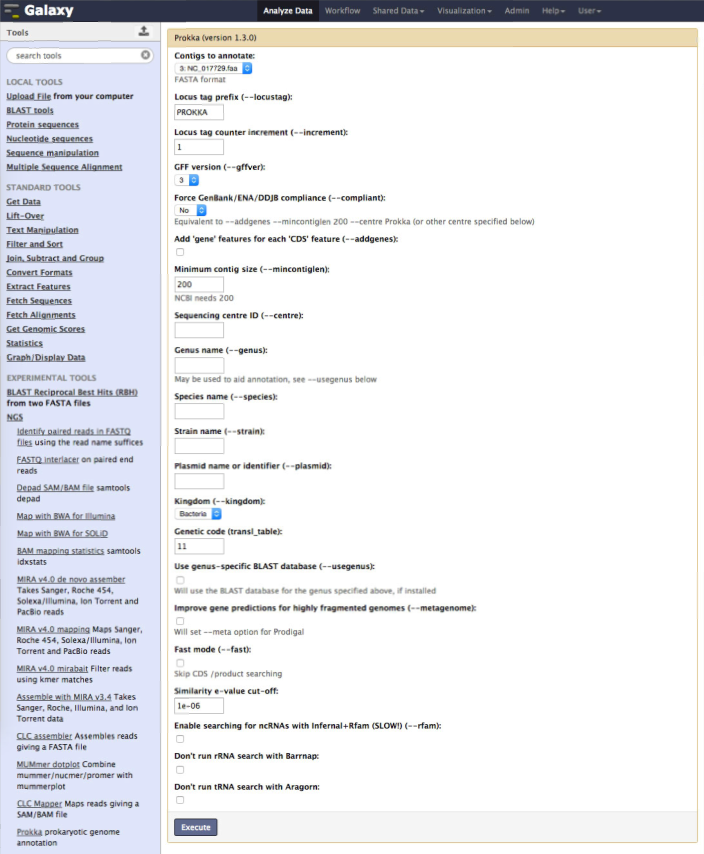
\includegraphics[width=0.9\textwidth]{images/prokka_galaxy}
    \end{column}
  \end{columns}
  Simple to run (at the command-line, or in \texttt{Galaxy}\footnote{\tiny{\href{http://dx.doi.org/10.1186/gb-2010-11-8-r86}{Goecks \textit{et al}. (2010) \textit{Genome Biol.} \textbf{11}:R86 doi:10.1186/gb-2010-11-8-r86}}}). \\
\end{frame}

% RAST
\begin{frame}
  \frametitle{RAST\footnote{\tiny{\href{http://dx.doi.org/10.1186/1471-2164-9-75}{Aziz \textit{et al}. (2008) \textit{BMC Genomics} \textbf{9}:75 doi:10.1186/1471-2164-9-75}}}}
  \begin{columns}
    \begin{column}{5cm}
      \begin{itemize}
        \item Server-based (\href{http://rast.nmpdr.org/}{http://rast.nmpdr.org/})
        \item Relies on SEED and FIGFam databases, held at NMPDR
        \item \textbf{FIGFam}: isofunctional homologue families
        \item Produces metabolic reconstruction
        \item Can be queues.
      \end{itemize}
    \end{column}
    \begin{column}{5cm}
      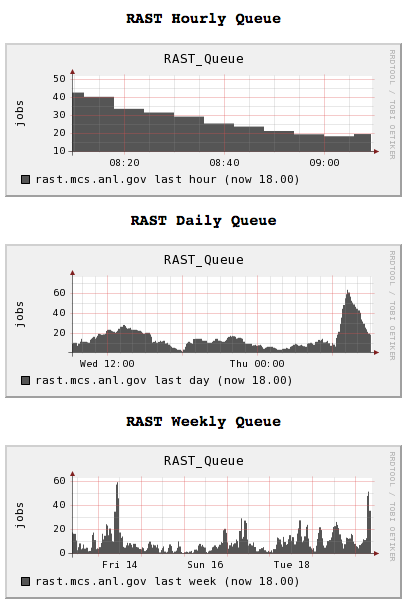
\includegraphics[width=0.9\textwidth]{images/rast_queue}
    \end{column}
  \end{columns}
\end{frame}